\subsection{Example \#4 -- when the LLN doesn't work}
We have two groups of students who have to take a math test. Group A has a mean score of 70 and a standard deviation of 10, while group B has mean 60 and standard deviation 20. Both groups have a normal distribution.
We take a sample of size $n$ from each group and calculate the sample means. Then, we calculate the difference between the sample means, $d_{AB}=\bar{x}_A-\bar{x}_B$, and the ratio between the means, $r_{AB}=\bar{x}_A/\bar{x}_B$.
As before, we increase the sample size and see how it affects $d_{AB}$ and $r_{AB}$.

\begin{knitrout}
\definecolor{shadecolor}{rgb}{0.969, 0.969, 0.969}\color{fgcolor}\begin{kframe}
\begin{alltt}
\hlstd{n} \hlkwb{<-} \hlkwd{seq}\hlstd{(}\hlnum{50}\hlstd{,}\hlnum{5000}\hlstd{,}\hlkwc{by}\hlstd{=}\hlnum{10}\hlstd{)}
\hlkwd{set.seed}\hlstd{(}\hlnum{59112}\hlstd{)}
\hlstd{allDiffs} \hlkwb{<-} \hlkwd{rep}\hlstd{(}\hlnum{0}\hlstd{,}\hlkwd{length}\hlstd{(n))}
\hlstd{allRatios} \hlkwb{<-} \hlkwd{rep}\hlstd{(}\hlnum{0}\hlstd{,}\hlkwd{length}\hlstd{(n))}
\hlkwa{for} \hlstd{(i} \hlkwa{in} \hlnum{1}\hlopt{:}\hlkwd{length}\hlstd{(n)) \{}
  \hlstd{sA} \hlkwb{<-} \hlkwd{rnorm}\hlstd{(n[i],}\hlnum{70}\hlstd{,}\hlnum{10}\hlstd{)}
  \hlstd{sB} \hlkwb{<-} \hlkwd{rnorm}\hlstd{(n[i],}\hlnum{60}\hlstd{,}\hlnum{20}\hlstd{)}
  \hlstd{dAB} \hlkwb{<-} \hlstd{sA} \hlopt{-} \hlstd{sB}
  \hlstd{rAB} \hlkwb{<-} \hlstd{sA} \hlopt{/} \hlstd{sB}
  \hlstd{allDiffs[i]} \hlkwb{<-} \hlkwd{mean}\hlstd{(dAB)}
  \hlstd{allRatios[i]} \hlkwb{<-} \hlkwd{mean}\hlstd{(rAB)}
\hlstd{\}}
\hlkwd{par}\hlstd{(}\hlkwc{mfrow}\hlstd{=}\hlkwd{c}\hlstd{(}\hlnum{1}\hlstd{,}\hlnum{2}\hlstd{))}
\hlkwd{plot}\hlstd{(n, allDiffs,}\hlkwc{pch}\hlstd{=}\hlnum{19}\hlstd{,}\hlkwc{col}\hlstd{=}\hlnum{3}\hlstd{,} \hlkwc{xlab}\hlstd{=}\hlstr{"n"}\hlstd{,} \hlkwc{ylab}\hlstd{=}\hlstr{"Diff."}\hlstd{,} \hlkwc{cex}\hlstd{=}\hlnum{0.5}\hlstd{)}
\hlkwd{abline}\hlstd{(}\hlkwc{h}\hlstd{=}\hlnum{10}\hlstd{,}\hlkwc{col}\hlstd{=}\hlnum{2}\hlstd{,}\hlkwc{lwd}\hlstd{=}\hlnum{2}\hlstd{)}
\hlkwd{plot}\hlstd{(n, allRatios,}\hlkwc{pch}\hlstd{=}\hlnum{19}\hlstd{,}\hlkwc{col}\hlstd{=}\hlstr{"orange"}\hlstd{,} \hlkwc{xlab}\hlstd{=}\hlstr{"n"}\hlstd{,} \hlkwc{ylab}\hlstd{=}\hlstr{"Ratio"}\hlstd{,} \hlkwc{cex}\hlstd{=}\hlnum{0.5}\hlstd{)}
\hlkwd{abline}\hlstd{(}\hlkwc{h}\hlstd{=}\hlnum{70}\hlopt{/}\hlnum{60}\hlstd{,}\hlkwc{col}\hlstd{=}\hlnum{2}\hlstd{,}\hlkwc{lwd}\hlstd{=}\hlnum{2}\hlstd{)}
\end{alltt}
\end{kframe}\begin{figure}

{\centering 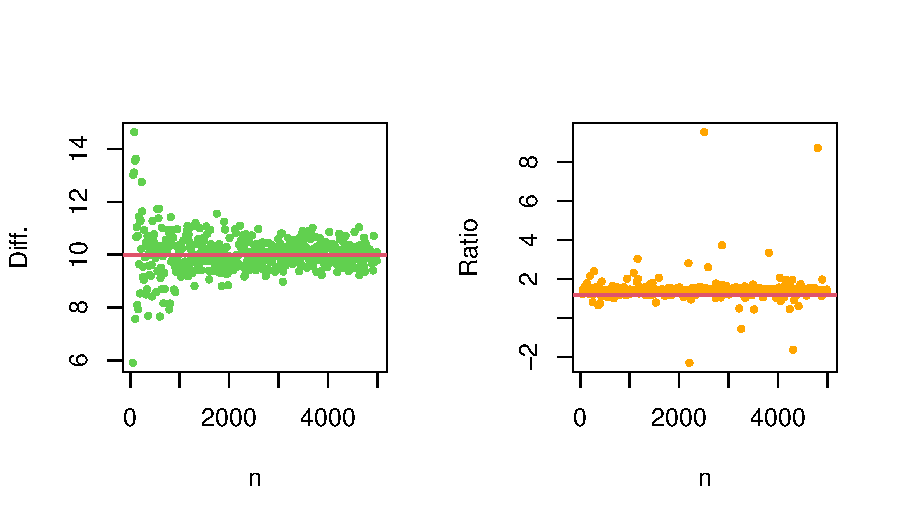
\includegraphics[width=\maxwidth]{figure/intro-lln4-0-1} 

}

\caption[Simulated test scores - difference and ratio between two groups]{Simulated test scores - difference and ratio between two groups.}\label{fig:intro-lln4-0}
\end{figure}

\begin{kframe}\begin{alltt}
\hlkwd{par}\hlstd{(}\hlkwc{mfrow}\hlstd{=}\hlkwd{c}\hlstd{(}\hlnum{1}\hlstd{,}\hlnum{1}\hlstd{))}
\end{alltt}
\end{kframe}
\end{knitrout}

What we see here is that the mean difference between the groups, $d_{AB}$, converges to the true difference between the groups (10), but the ratio, $r_{AB}$, does not converge -- $n$ can be as large as we want, and we will still see ratios that are quite extreme. (Note that the mean of a ratio between two distributions is generally not equal to the ratio of the means of the distributions, so we don't expect $r_{AB}$ to converge to exactly 70/60.)

What is happening here? The answer is that while a difference between two normal random variables is still normal (and hence, has a mean), the ratio between two normal distributions follows a Cauchy distribution which doesn't have a theoretical mean, so the LLN does not apply to  $r_{AB}$.

Although the LLN applies to almost any distribution we will ever encounter, the lesson here is that taking the ratio between two perfectly well-behaved distributions may lead to a distribution to which the LLN does not apply. Other manipulations of random variables may lead to similar results.
